%\documentclass{svjour3}                     % onecolumn (standard format)
%\documentclass[smallcondensed]{svjour3}     % onecolumn (ditto)
\documentclass[smallextended]{svjour3}       % onecolumn (second format)
%\documentclass[twocolumn]{svjour3}          % twocolumn

\smartqed  % flush right qed marks, e.g. at end of proof

% \usepackage{mathptmx}      % use Times fonts if available on your TeX system

% insert here the call for the packages your document requires
\usepackage[utf8]{inputenc}
% Use nameref to cite supporting information files (see Supporting Information section for more info)
\usepackage{nameref,hyperref}
% amsmath and amssymb packages, useful for mathematical formulas and symbols
\usepackage{amsmath,amssymb}
% useful for consistent display and control of units of measurement
\usepackage{siunitx}
% figures!
\usepackage{graphicx}
% for including TODO notes
\usepackage{todonotes}
% snyntax highlighting for code
\usepackage{minted}
% manually set margins
\usepackage{geometry}[margins=1in]
%

\journalname{Sports Engineering}

\begin{document}

\title{Analysis and Ethical Design of Terrain Park Jumps for Snow Sports}

\author{Jason K. Moore      \and
        Bryn Cloud          \and
        Mont Hubbard        \and
        Christopher Brown
}

%\authorrunning{Short form of author list} % if too long for running head

\institute{J.K. Moore \at
              Delft University of Technology \\
              Tel.: +123-45-678910\\
              \email{j.k.moore@tudelft.nl}           %  \\
%             \emph{Present address:} of F. Author  %  if needed
           \and
           S. Author \at
              second address
}

\date{Received: date / Accepted: date}
% The correct dates will be entered by the editor

\maketitle

\begin{abstract}
  Terrain parks now exist at almost all United Stats snow sport resorts. For
  several decades, epidemiological evidence shows increased injuries correlate
  with terrain park use. Injury risk could be reduced through analytical
  engineering design of jump profiles to control the equivalent fall height,
  i.e., energy dissipated on impact when landing. We know of no evidence the
  ski industry and their insurance companies are supporting making terrain park
  jumps safer in this way. We discuss two case studies illustrating that large
  equivalent fall heights play significant roles in traumatic injuries in
  terrain park jumps. As a remedy, we provide an accessible online tool for
  terrain park builders, both to evaluate safety of existing jumps by
  calculating their impact danger and to design jump profile shapes that
  control equivalent fall heights and thereby reduce the risk of injury.
\end{abstract}

\section{Introduction}
\label{intro}
%
When a falling person impacts a fixed surface, there is risk of injury. Greater
impact velocity normal to the surface will inevitably cause greater injury, due
to increased kinetic energy that must be dissipated on impact. A common
surrogate for measuring impact energy is ``equivalent fall height'', a
conceptually simple and familiar interpretation of impact danger used in a
variety of safety standards around the world, from construction~\cite{OSHA2021}
to children's playground equipment~\cite{Chalmers1996}. The equivalent fall
height of ski and snowboard terrain park jumps can be
calculated~\cite{McNeil2012} if the Cartesian coordinates of the jump profile
are known, including the starting point, take off ramp, and landing hill along
the jumper's path. Controlling energy dissipation in the human body, and hence
controlling equivalent fall height in terrain park jumps, is paramount to safe
design methods to reduce likelihood and severity of injury. Equivalent fall
height should be a primary attribute of a jump's landing design taken into
consideration because of this clear connection to injury risk and the ease of
which it can be controlled for.~\todo{Maybe we should also mention that
shortening the approach, and thus max possible speed, is the first and simplest
adjustment for decreasing injury - JM}.

This paper discusses societal costs of increasing terrain park injuries and
focuses on two case studies that illustrate the danger if equivalent fall
height is not controlled. Following this, we highlight examples of published
ski safety research that attempt to sow doubt instead of contributing to
improved safety. We then present a user-friendly web application for
calculating equivalent fall height of existing or planned jumps. We see this
application as a part of the solution to reducing injuries in terrain park
jumps. Jump builders may use it to reduce the risk of injuries in their
resorts.

\subsection{History}
\label{sec:hist}
%
Terrain park jumps are not new additions to snow sports resorts. Their gradual
introduction in the 1980's was tied to increased interest in aerial maneuvers
and extreme sports participation. Growth accelerated and has continued. Today
nearly 95\% of US ski resorts include terrain parks. Unfortunately, this
ubiquity is correlated to injury increases. Two early longitudinal studies in
the 1980's and early 1990's~\cite{Deibert1998,Furrer1995} had already found
significant increases in head injuries and concussions. The Consumer Product
Safety Commission determined that between 1993 and 1997 head injuries accounted
for a majority of skiing and snowboarding deaths~\cite{CPSC1999}. An early
review~\cite{Koehle2002} noted that ``[S]eventy-seven percent of spinal
injuries~\cite{Tarazi1999} and 30\% of head injuries~\cite{Fukuda2001} in
snowboarding were a result of jumps.'' Jackson et al.~\cite{Jackson2004}
determined that by 2004 snow skiing had replaced football as the second leading
cause of serious head and spinal cord injuries in the US.

These early increasing injury assessments persisted. According to
\cite{Russell2014}, ``between 5\% and 27\% of skiing and snowboarding injuries
occur[red] in terrain parks
\cite{Bridges2003,Goulet2007,Moffat2009,Greve2009,Brooks2010,Ruedl2013}''.
Incredibly, at the first Winter Youth Olympic Games more than a third of all
snowboard half-pipe and slope-style competitors became
injured~\cite{Ruedl2012}. Epidemiological research continues to show
\cite{Carus2016,Audet2019a,Hosaka2020} that injuries on terrain park jumps are
both more likely and more severe than those on normal slopes. Audet et.
al~\cite{Audet2019a} states there is strong evidence that skiing or
snowboarding in a terrain park is a risk factor for head, neck, back, and
severe injuries. Hosaka et. al~\cite{Hosaka2020} concludes that jumping is one
of the main causes for serious spinal injuries, regardless of skill level, and
suggests that, because the incidence of spinal injuries has not decreased over
time, ski resorts and the ski industry should focus on designing fail-safe jump
features to minimize the risk of serious spinal injury. Similar suggestions
have repeatedly been made in peer-reviewed literature for more than a
decade~\cite{Hubbard2009,Swedberg2012,McNeil2012,McNeil2012a,Hubbard2015,Levy2015,Petrone2017,Moore2018}.

\section{Equivalent Fall Height}
\label{sec:efh}
%
\emph{Equivalent fall height}, the kinetic energy that must be dissipated on
impact from a given height, is a common proxy measure for impact danger by
industry in safety standards~\cite{Hubbard2012}. On the earth's surface this
energy is given by the well known equation $mgh$ and is equal to the kinetic
energy available to injure a person in a non-rotating fall. The ability of this
energy to injure can be reduced by controlling impact circumstances, e.g.
impact cushioning, body orientation, body configuration and active body motion;
however this energy must still be dissipated. Larger equivalent fall heights
require more elaborate protection measures to reduce injury whereas lowering
equivalent fall height is a non-elaborate measure for increasing safety.

Equivalent fall height is a particularly useful measure of danger due to its
interpretability by lay people. People have an intuitive danger sense when
faced with potential falls from large heights and they have strong common sense
for relating fall height to likelihood of injury due to experience with their
own and others' falls. For example, we have a sense of the danger associated
with falling from building stories of increasing magnitude. Ground floor falls
are on the order of 2.6~\si{\meter}, second story are 5.1~\si{\meter}, third
story 8.8~\si{\meter}, and so on~\cite{Vish2005}. The US Occupational Safety
and Health Administration, OSHA, requires fall protection for fall heights
greater than 1.2~\si{\meter} for general workplace safety~\cite{OSHA2021}.
Chalmers et al.~\cite{Chalmers1996} argues for 1.5~\si{\meter} maximum fall
heights for playground equipment. The Swiss Council for Accident Prevention
make specific recommendations for equivalent fall height to be lower than
1.5~\si{\meter} for jumps requiring basic skills~\cite{Heer2019}. And although
there are no standards in Olympic Nordic ski jumps, ``equivalent landing
height`` is used in their design~\cite{Gasser2018} and these heights have been
measured to be in the neighborhood of 0.5~\si{\meter}.

The equivalent fall height $h$ of an object is formally defined as
%
\begin{equation} h = \frac{v^2}{2g} \label{eq:efh_general} \end{equation}
%
where $v$ is the impact velocity of the object and $g$ is the acceleration due
to gravity. This definition results from equating the kinetic energy of an
object moving at velocity $v$ at impact with the potential energy of the same
object at height $h$ above the ground.

Using Equation~\ref{eq:efh_general} as a starting point, the equivalent fall
height $h$ can be determined for any landing surface one impacts after a jump
flight trajectory~\cite{Petrone2017}. The resulting equation, neglecting air
drag here for simplicity, is
%
\begin{equation}
  h = \left[\frac{x^2}{4(x\tan\theta_T - y)\cos^{2}\theta_T} -
    y\right]\sin^{2}\left[\tan^{-1}\left(\frac{2y}{x}- \tan\theta_T\right) -
    \tan^{-1}\frac{dy}{dx}\right]
  \label{eq:efh}
\end{equation}

This expression is  a function of only four variables: takeoff angle
$\theta_T$, impact coordinates $(x,y)$ on the landing surface, and the slope of
the landing surface $\frac{dy}{dx}$. Note that the expression is not a function
of takeoff speed~\cite{Petrone2017}. To analyze a jump, it is sufficient to
measure the Cartesian coordinates of the landing surface along the jumper's
flight path and the takeoff angle. Slopes $\frac{dy}{dx}$ are computed
numerically from the measured coordinates $(x,y)$.
%~\todo{LET'S EXPLAIN WHY SPEED CAN BE IGNORED -- CB}. the ref does this- MH

\section{Case Studies}
\label{sec:case}
%
Next we present two case studies from court proceedings in the United States.
In both these cases juries ruled in favor of injured plaintiffs, judging that
neglect in jump design and construction contributed significantly to the
injuries~\cite{Alvarado2002,Salvini2008}. The simulation results below follow
from the methods in \cite{Levy2015} and assume skier mass, frontal area, and
drag coefficient of 75~\si{\kg}, 0.34~\si{\meter\squared}, and 0.821,
respectively.

\subsection{Vine v. Bear Valley}
\label{sec:vine}
%
In April 2000, Ms.~Vine's lower spine was injured when she fell on a jump at
Bear Valley Ski Resort in California. The jump shape
(Fig.~\ref{fig:vine-v-bear-valley}) was a common form of terrain park jump
called a ``table-top''. The builder's intent is that jumpers completely clear
the table, landing on the down-slope near the so-called ``sweet spot'', but
Vine landed short of the knuckle (the end of the table-top). The upper panel of
Fig.~\ref{fig:vine-v-bear-valley} shows the jump surface from accident
investigation measurements. This table-top, which would typically be flat and
horizontal, was instead concave, compounding the danger of a short landing. At
the 11~\si{\meter} actual measured horizontal landing distance from the takeoff
point, the surface was sloped upwards approximately 5~\si{\degree}. The concave
shape emphasizes the detrimental effect of not aligning more closely the
surface tangent with the jumper flight path at impact.
%
\begin{figure}
  \centering
  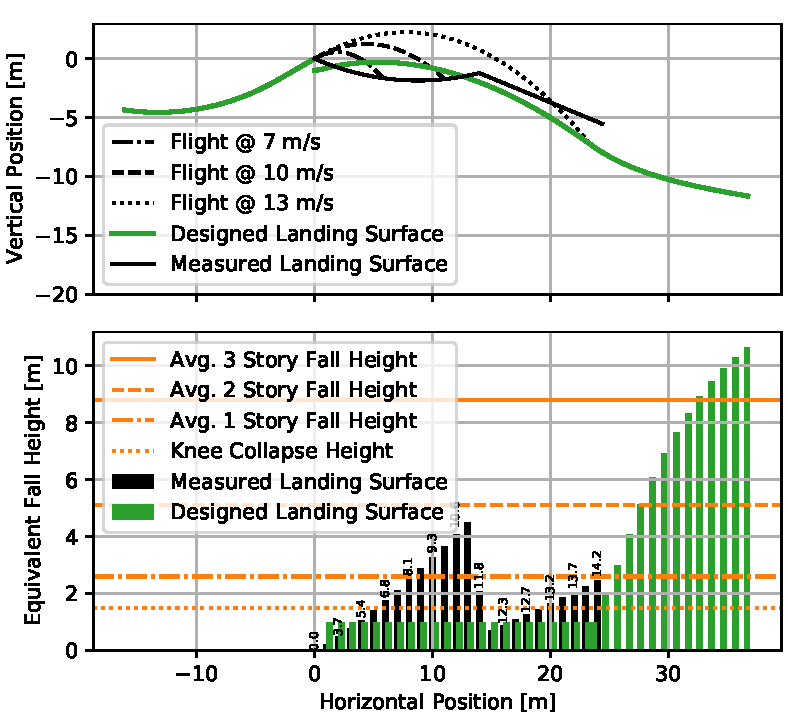
\includegraphics[width=5.25in]{figures/vine-v-bear-valley.pdf}
  \caption{\textbf{Bear Valley jump compared to possible safer design}
  Top: Measured landing surface (solid black) and jumper flight paths
  (intermittent black) from measured 30\si{\degree} takeoff angle. The
  14~\si{\meter\per\second} takeoff speed is used as the design speed \cite{Levy2015} for a
  comparison jump (solid green) shaped to have constant equivalent fall
  height of 1~\si{\meter}.
  Bottom: Equivalent fall height for both jumps in corresponding
  colors at 2~\si{\meter} intervals. Numbers above bars indicate
  takeoff speeds required to land at that location.
  Intermittent horizontal gray lines indicate relatable fall heights: knee
  collapse, average 1st story fall, and average 2nd story fall.
  }
  \label{fig:vine-v-bear-valley}
\end{figure}

The lower panel displays equivalent fall height at different landing locations.
It is clear that just short of the knuckle, equivalent fall height is highest.
At the ``sweet spot'' just past the knuckle the equivalent fall height drops
precipitously to  about 1~\si{\meter} but landing in this narrow region
requires the jumper to control take-off speed to better than
1~\si{\meter\per\second} precision. At a landing distance of 11 meters, Vine's
fall height would have been almost 4 meters, equivalent to falling from between
one and two stories~\cite{Vish2005}. Vine's body had also rotated backward in
flight. She landed on her lower spine and was paralyzed as a result of the
nearly two story fall. A lower equivalent fall height would have decreased the
possibility of spinal injury, due to the lower impact forces when landing in
the rotated position.

In contrast, a landing surface designed to have a smaller constant equivalent
fall height can be created with a similar amount of construction costs. The
green jump profile in the upper panel of Fig.~\ref{fig:vine-v-bear-valley}
shows a possible jump design, see~\cite{Levy2015}, of similar size with similar
flight times that ensures a constant (smaller) equivalent fall height almost
everywhere of 1~\si{\meter}. The convex shape of this jump is interestingly
close to what one would get if the original concave table-top were inverted,
showing how the convex nature of the landing shape is critically important to
control equivalent fall height. This jump design would have lowered impact
forces for landings at any location. In 2002, the jury ruled in favor of
Ms.~Vine, agreeing that Bear Valley was responsible for designing safer jumps.

\subsection{Salvini v. Ski Lifts Inc.}
\label{sec:salvini}
%
In 2004, Mr.~Salvini attempted a table-top jump on skis in the terrain park of
The Summit at Snoqualmie Ski Resort, in Washington state. Salvini overshot the
intended landing location while traveling at typical skiing speeds, rotated
backward during flight and landed on his back, ultimately suffering
quadriplegia.  At his landing location the equivalent fall height was over 10
meters, approximately a 3-story fall. Figure~\ref{fig:salvini-v-snoqualmie}
shows the jump profile based on measurements from the accident investigation.
For takeoff speeds greater than 13~\si{\meter\per\second}, the lower panel
shows that the equivalent fall height is greater than 10~\si{\meter} and grows
linearly with larger takeoff speeds. Severe injury is almost certain in falls
this high, especially so if landing in a way that causes undue forces to the
spine, as in this case.

The upper panel also shows a jump profile (green) designed to have a
1~\si{\meter} equivalent fall height for all speeds below
16~\si{\meter\per\second}. This profile requires significantly more snow than
the measured jump but alleviates the dangerous impacts possible in the measured
jump.

This jump highlights how extreme the equivalent fall height can become if the jump
is not properly designed. Few recreational skiers will jump out of a three
story window, snow landing or not. The likelihood of injury is quite clear and
our internal altimeter tells us so. However, our internal altimeters cannot
sense potential risks until we have left the takeoff and are in the air.
%
\begin{figure}
  \centering
  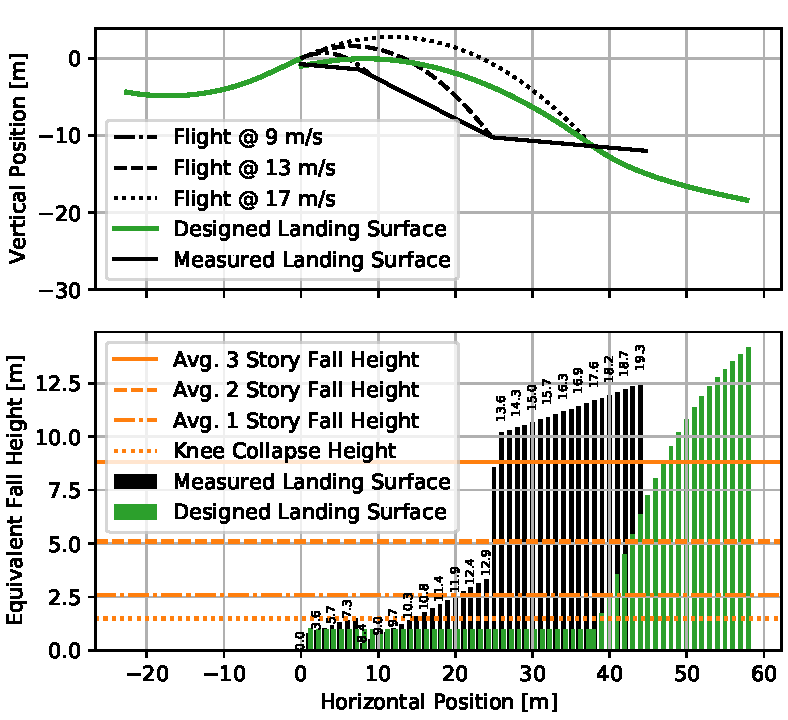
\includegraphics[width=5.25in]{figures/salvini-v-snoqualmie.pdf}
  \caption{\textbf{Snoqualmie jump compared to possible safer design}
  Top: Measured landing surface (solid black) and jumper flight paths
  (intermittent black) for measured 25\si{\degree} takeoff angle. The
  16~\si{\meter\per\second} takeoff speed is used as the design speed for a
  comparison jump (solid green) with constant equivalent fall height of
  1~\si{\meter}.
  Bottom: Equivalent fall height for both jumps in corresponding colors
  at 2~\si{\meter} intervals. Numbers above bars indicate takeoff speed
  required to land at that location.
  Intermittent horizontal gray lines indicate relatable fall heights: knee
  collapse, average 1st story fall, average 2nd story fall, and average 3rd
  story fall.
  }
  \label{fig:salvini-v-snoqualmie}
\end{figure}


These two case studies clearly show that no or poor jump design can cause
devastating consequences and that engineering analysis and design, based on the
laws of mechanics, can be used to shape jump landings that limit equivalent
fall height. Designing jumps in this way is based on the well-established,
centuries-old physics of Issac Newton and Émilie du Châtelet~\cite{Zinsser2007}
which are fundamental to engineering education. It is really irrefutable that
designing jumps can reduce injury risk by limiting equivalent fall height and
hence the amount of impact energy dissipation.

\section{Moral Imperative}
\label{sec:moral}
%
Employing engineering to reduce the risk of injury on fabricated terrain park
jumps motivates this work. Our motivation is consistent with the first canon of
engineering ethics: ``Hold paramount the safety, health and welfare of the
public''~\cite{NSPE2019}. In the context of snow sport safety, the first canon
compels engineers to direct their technical expertise to protecting snow sport
participants from injuries. No one can rationally argue that reducing
equivalent fall height would cause an increased likelihood of injury and, if
shaping designed jump landing surfaces is no more laborious than shaping
non-designed surfaces, therefore there can be no reason not to control
equivalent fall height. Then what explains the reluctance of the skiing
industry and their insurance companies to adopt such design methods?

Oreskes and Conway~\cite{Oreskes2010} have studied this problem more generally.
They have shown that from time to time, scientific evidence accumulates that
certain commonly occurring industrial activities are harmful, either to
individuals or to society as a whole. Nearly always the industries have a
vested interest in continuing the status quo, since operational changes likely
will lead to significant financial or other costs. Examples of such situations
over the last 60 years exhaustively described and analyzed in
~\cite{Oreskes2010} are the use of DDT, smoking tobacco, acid rain linked to
coal-fired power plants, the ozone hole caused by CFCs, second-hand tobacco
smoke’s effects, and CO2-caused climate change, among others. Rather than using
the proven science as a basis for changes in practice, the common strategic
response of the industries involved has been to “emphasize the controversy
among scientists and the need for continued research”~\cite{Oreskes2010}. A
similar strategy has been used by skiing defense experts. To counter the solid,
fundamental, scientific concept of landing surface design based on equivalent
fall height, defense experts have introduced confounding factors that serve to
cloud and confuse the basic issues.  Consider three examples of papers
co-authored by well-known skiing industry defense experts who have testified
for the skiing industry and their insurance companies.

~\todo{Not sure this paragraph still should be included. It is relevant but maybe  distracting.}
People unfamiliar with the legal and insurance systems in the USA may fail to
appreciate that technical literature is often corrupted in legal defense of
unsafe practices and to protect corporate assets. Peer-reviewed technical
literature is often used to support testimony in U.S. lawsuits. Both plaintiffs
and defendants hire their own experts to testify and authors of technical
papers can make money by testifying. When this testimony is for the defense, it
can result in denying compensation for injuries, and serve to prolong unsafe
practices. Rarely do experts report conflicts of interest in their papers and
presentations, or when they organize and chair meetings or edit publications.
Financial support for publications used by expert witnesses can be routed
through consulting companies to pretend plausible deniability of conflicts of
interest in their papers. Sadly, this is deceitful, self-serving, and
unethical, because it ignores the first canon of engineering ethics. It could
be argued that, if someone ignores engineering ethics, they are not acting as
engineers, and what they are doing cannot be considered engineering.

Shealy et. al~\cite{Shealy2010} conducted an experimental study which attempts
to test the hypothesis that takeoff speed is a predictor of the distance from a
take-off to a jump landing. They indicate that a series of jumpers who use a
terrain park jump land within a narrow region, which is reasonable once it is
noted that the jumpers' takeoff speeds did not vary much either, i.e. no
attempt was made to assess a reasonable range of their independent variable,
speed. The authors state the preposterous conclusions both that there is ``no
statistically significant relationship between takeoff speed and the distance
traveled'' and that ``takeoff speed is not a dominant or controlling factor (in
how far a jumper travels)''. These results should lead the careful researcher
to question their experimental design and analysis methods, just as a high
school physics student should if their an object in their lab experiment does
not fall with an acceleration close to 9.8~\si{\meter\per\second\squared}.

Shealy et. al~\cite{Shealy2015} claim that catastrophic and fatal injury rates
at US snow resorts have not changed, even though terrain parks (and thus likely
jumping) have increased over time. The statistical model in this study was
expressly designed such that passage of time was used as the sole explanatory
variable for incident rates. The authors do not report absolute numbers of
fatalities and injuries, only incident rates, which provide a more favorable
view for the ski industry and their risk assessment. No data is disclosed and
they use unspecified weighting factors in order to harmonize data over time,
leaving one to question what these weightings are. Data and robust modern
statistical methods exist for testing their stated hypothesis. We can only
speculate as to why those may have not been used for this analysis. Drawing
their final conclusion, that addition of terrain parks mitigates risks, is
quite a stretch, given the data and debatable analysis. When it comes to health
and safety of the public, society is also interested in reducing or eliminating
the absolute numbers.  This is especially true for activities in which the risk
of catastrophic life-changing or fatal injuries can be mitigated by ethical
engineering designs, and therefore are not be inherent to the sport.

In an article on landing positions, Scher et. al show that body orientation at
impact can cause dangerous cervical spine loads~\cite{Scher2015}. They report
on effects of equivalent fall height but only test heights from
\SIrange{0.23}{1.52}{\meter}, both committing a similar fault as in by
\cite{Shealy2010} restricting the range of their independent variable
inappropriately, and not testing fall heights that are known to have caused
severe injury. Yet the authors purport that equivalent fall height has no
appreciable effect on injury. The title of this paper, ``Terrain Park Jump
Design: Would Limiting Equivalent Fall Height Reduce Spinal Injuries?'' implies
that the authors may believe falling on ones head from greater and greater
heights may \emph{not} cause greater injuries. It is not clear why one might
propose such a hypothesis in the first place.

The first two studies do a poor job of isolating variables, and apparently were
not intended to, and the third suffers from restriction of equivalent fall
height range. But most importantly, and quite noticeably, none of these papers
are written with the intent to reduce injury rates. No ways are suggested in
which their findings could be used to promote the safety, health, and welfare
of the public. What these papers have done, is attempt to muddy the waters
regarding the fact that impacting a surface at a lower velocity is safer. This
strategy of introducing bogus science is well known in litigation in the U.S..
For example the same strategy was used to defend the tobacco
industry~\cite{Oreskes2010}.

Poorly executed experiments in snow sports or elsewhere, no matter how
expensive and sophisticated the instrumentation, cannot disprove the
fundamental laws of mechanics. If statistics or experimental results do seem in
conflict with predictions from classical mechanics, then there is likely a
problem with the statistical or experimental design or its interpretation, and
not with the mechanics itself. Defending practices that lead to injuries at the
service of protecting corporate assets can prolong these practices, which can
lead to further injuries, clearly violating the first canon of engineering
ethics.

Testifying for an injured plaintiff, or to defend corporations, in injury
cases, are not equivalent actions ethically. Authoring papers with no intent on
improving safety and reducing injuries is unethical. One attempts to address
problems that cause injuries, holding paramount the safety health and welfare
of the public. The other attempts to defend the practices that might have
contributed to the injury, in order to limit financial losses of insurance
companies. The proverbial two sides to every question do not exist in science
and engineering.


use UPTON SINCLAIR quote \cite{Sinclair1994}
 “It is difficult to get a man to understand something, when his salary depends on his not understanding it.” 

\section{What Can Be Done?}
\label{sec:action}
%
Assessing and reshaping existing jumps for dangerous equivalent fall heights
should be an easy way for ski resorts to reduce the danger of their terrain
park jumps. Accurate enough measurements of an existing slope can be taken with
simple tools, e.g. a tape measure and a digital level, and only takes a short
amount of time per jump, see Appendix~\ref{sec:jump-shape-measurement}.  The
calculation and visualization of the equivalent fall height from these
measurements can take some time if manually done. A program for calculating
equivalent fall heights from a hill profile is now available as an online,
freely accessible, and user friendly web application that makes the calculation
and visualization step almost instantaneous for the terrain park builder. With
the tool described in the next section, terrain park builders can easily add
this safety assessment to their toolbox, even using it from a smartphone while
in the field. There is no reason that this basic assessment should not be part
of the jump construction process. The laws of nature clearly tell us that
designing jumps with lower equivalent fall heights will have a positive
probability in reducing injuries. The only ethical decision is to adopt these
methods; as saving even one person from a life of paralysis, or even death,
must be worth the minor inconvenience of shaping jumps using the rules in
\cite{Levy2015}.

\todo[inline]{Add:
Standards - ASTM F27,
Talk about how it was a long struggle to write ski binding adjustment standards,
The ski people forced a modified scope to avoid writing standards on snow surfaces,
Insurance and risk}

\subsection{Software and Online Access}
\label{sec:software}
%
We presented the first version of software for designing ski jumps with a
constant equivalent fall height in \cite{Moore2018}. The software comprises of
a general purpose, extensible, object oriented software library with tools for
2D skiing simulation. Using the library code, a web application was developed
for interactive jump design. The web application is designed for a
non-technical end user and usable on a desktop, tablet, or mobile device; any
device that supports a web browser.

We have extended the capabilities of the software in version 1.4.0, released
alongside this publication, for the purposes of the work described in this
paper. New library features were added that automate the calculation of
equivalent fall height for jump profiles described by a series of Cartesian
coordinates. Additionally, a new ``analysis'' page was added to the web
application which allows users to upload either a comma separated value CSV
text file or a Microsoft Excel spreadsheet file with the measured jump profile
coordinates. The jump is then analyzed and the equivalent fall height is
displayed graphically for interactive user manipulation and viewing.
Figure~\ref{fig:web-app-screenshot} shows the web application with one of the
case study jumps loaded for analysis and explains the primary features.
%
\begin{figure}
  \centering
  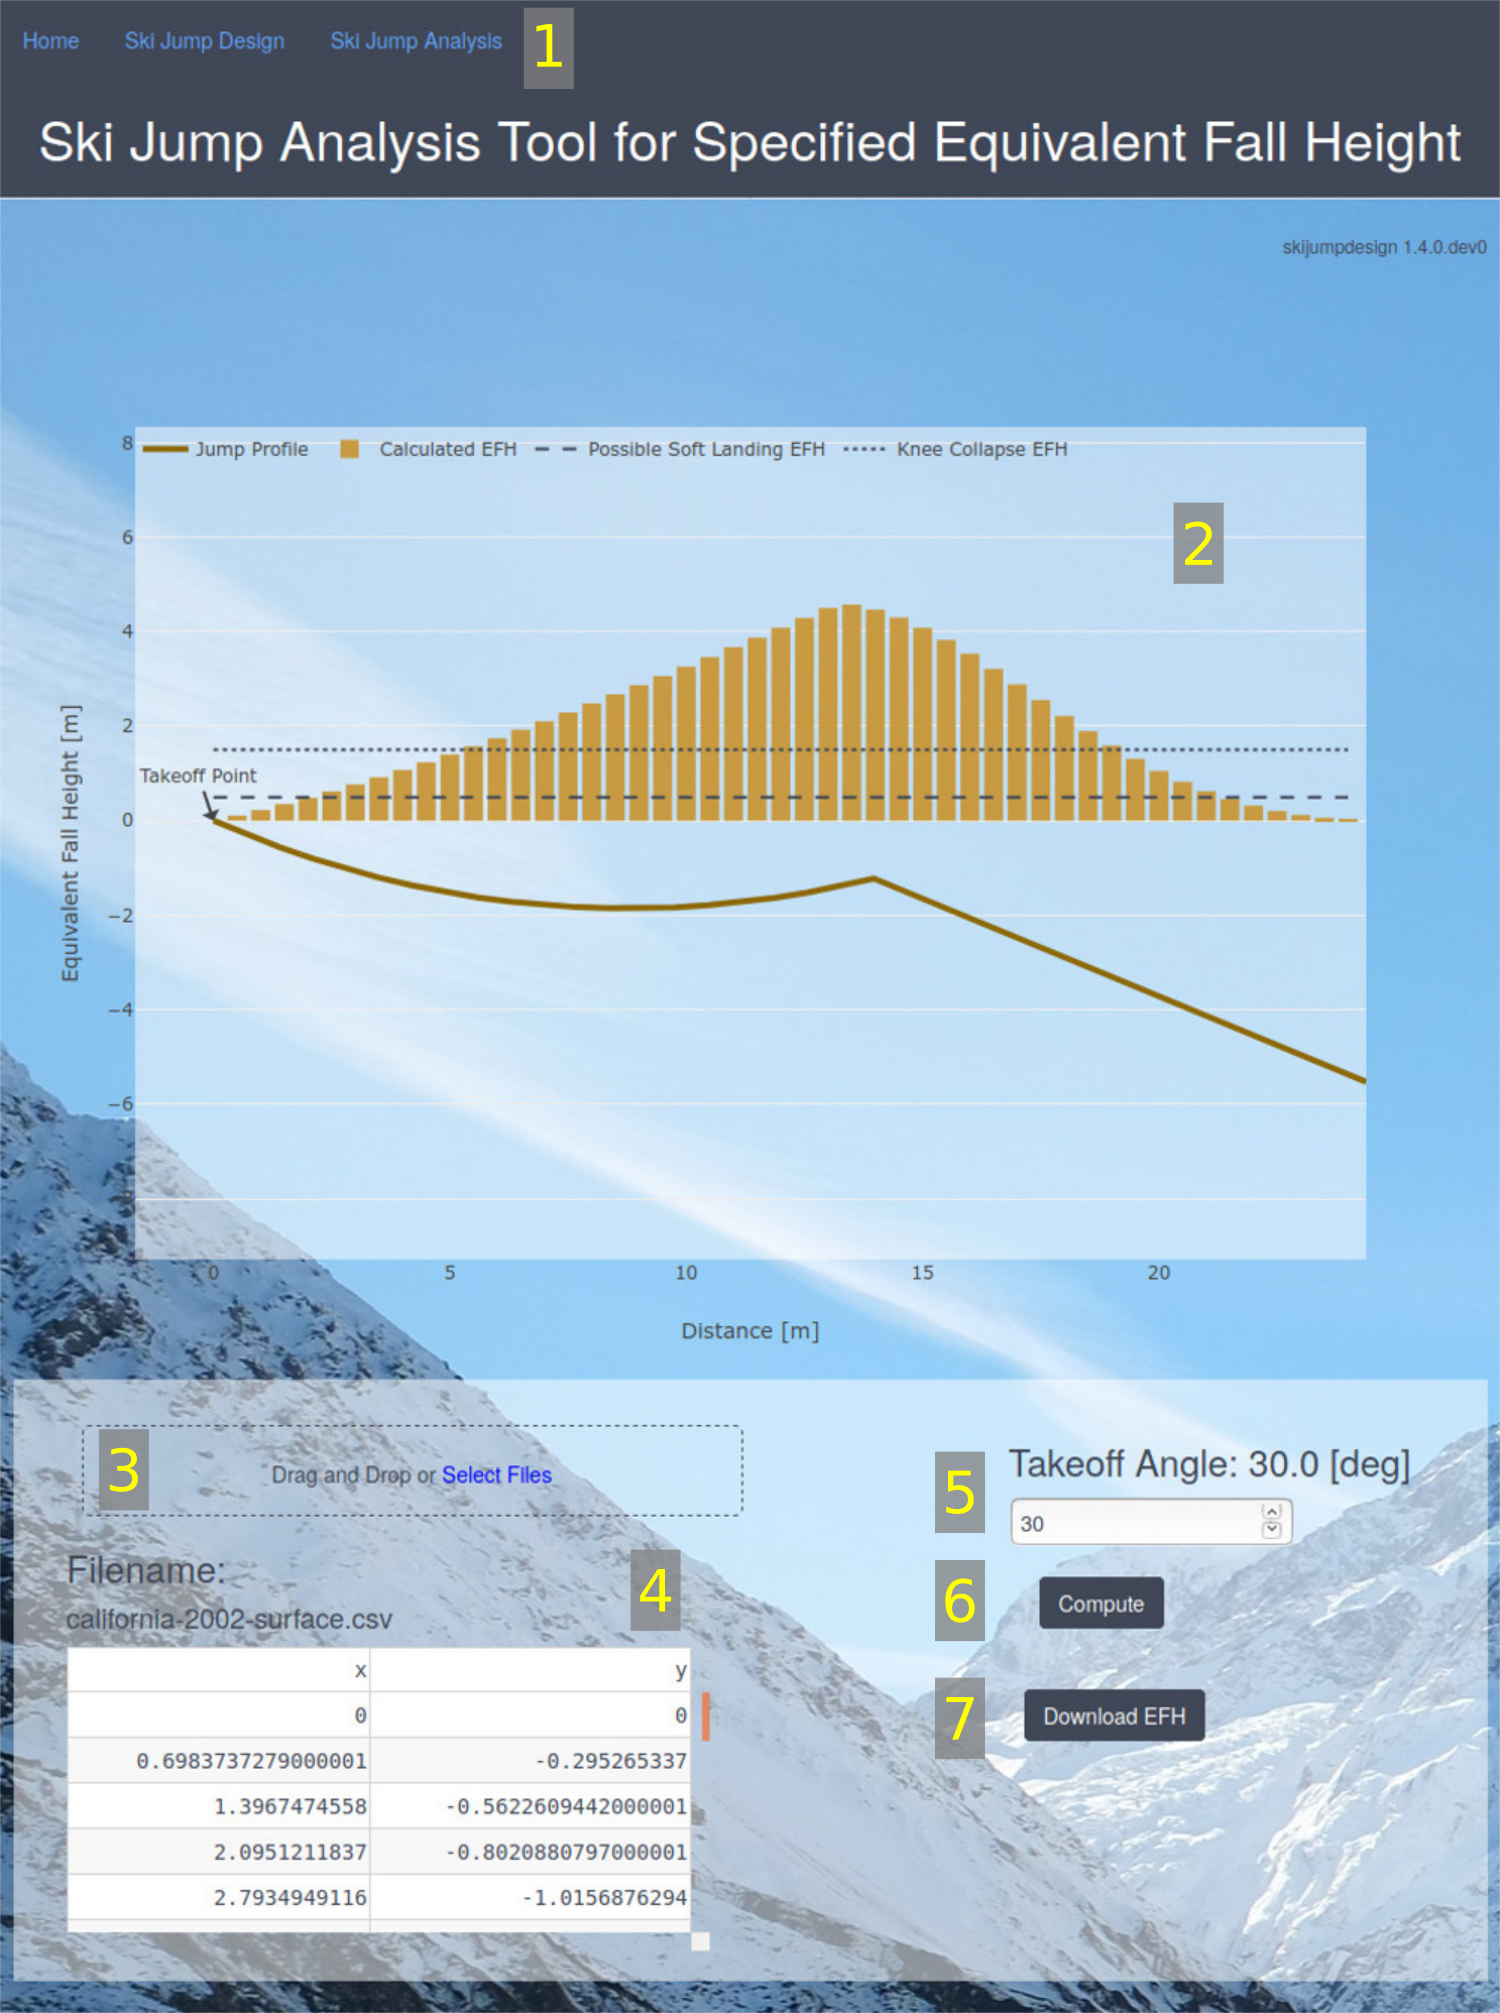
\includegraphics[width=5.00in]{figures/web-app-screenshot.png}
  \caption{\textbf{Screenshot of the ski jump design and analysis web app} To
    use the analysis portion of the app, a user selects ``Ski Jump Analysis''
    from the primary menu [1], uploads a CSV or XLS file by dragging it onto
    the screen [3], inspects the input data for accuracy in the table [4], sets
    the takeoff angle [5], runs the analysis by pressing the ``Run Analysis''
    button [6], views the results in the interactive plot [2], and downloads
    the results by pressing the ``Download EFH'' button [7].}
  \label{fig:web-app-screenshot}
\end{figure}

The software is written in Python and directly depends on popular packages
including Cython~\cite{Behnel2011}, matplotlib~\cite{Hunter2007},
NumPy~\cite{Oliphant2006}, pandas~\cite{McKinney2020},
Plotly/Dash~\cite{Plotly2015}, pycvodes~\cite{Dahlgren2018},
SciPy~\cite{Virtanen2020}, SymPy~\cite{Meurer2017}, and xlrd. The software is
open source and licensed under the MIT redistribution license. The source code
is available on Gitlab (\url{https://gitlab.com/moorepants/skijumpdesign}) and
PyPi (\url{https://pypi.org/project/skijumpdesign/}. Users can submit bug
reports, feature requests, code improvements, and additions at the Gitlab
repository. The software library is documented at
\url{https://skijumpdesign.readthedocs.io}. Basic examples of using the library
are provided in the documentation and this paper's appendix. The web app is
hosted for free use at \url{http://www.skijumpdesign.info}.

\section{Conclusion}
\label{sec:conc}
%
There are, of course, more factors than jump landing surface shape that
contribute to injuries on terrain park jumps but impact velocity can be easily
controlled with a designed landing surface. There is no evidence to support
that decreasing equivalent fall height increases injuries in falls, only
evidence that injuries can be decreased. Thus there is no reason not to adopt
constant equivalent fall heights of low values for public use jump designs.
Common sense is really all that is needed to believe that falling from higher
heights will increase injury to human bodies regardless of other factors. Any
person that must fall would surely choose to do so from the lowest height.
Constructors of terrain park jumps that are not designed with these facts in
mind are negligent. The safety, health, and welfare of the public involved in
this sport should be held paramount.

\begin{acknowledgements}
If you'd like to thank anyone, place your comments here
and remove the percent signs.
\end{acknowledgements}

% Authors must disclose all relationships or interests that 
% could have direct or potential influence or impart bias on 
% the work: 
%
\section*{Conflict of interest}
\label{sec:conflict}
%
The authors declare that they have XXXX.

% BibTeX users please use one of
%\bibliographystyle{spbasic}      % basic style, author-year citations
%\bibliographystyle{spmpsci}      % mathematics and physical sciences
%\bibliographystyle{spphys}       % APS-like style for physics
%\bibliography{}   % name your BibTeX data base

\bibliographystyle{spphys}
\bibliography{references}

\appendix

\section{Example software library use}
\label{sec:example}

%
The closed form equation~\ref{eq:efh} is useful for understanding the fundamental
relationship of equivalent fall height to the landing surface and well predict
these values for small jumps but other factors may be useful to include in the
model. For example, jumpers are subject to aerodynamic drag and this is not
negligible for larger jumps. If drag is included there is no closed form
solution for the equivalent fall height, but the equivalent fall height can be
computed through iterative simulation~\cite{Levy2015}. The jumper's flight path
is found by integrating the flight equations of motion at various takeoff
velocities and computing the misalignment in jumper landing angle and the slope
angle to then find the equivalent fall height. This more general simulation
method is implemented in the software described herein and the results reflect
the inclusion of gravitational and drag forces. The simulations require
measurements of the landing surface cross-sectional profile coordinates $(x,y)$
relative to the takeoff point and a measurement of the takeoff angle.

Listing~\ref{lis:example-efh-calc} demonstrates creating a surface from some
measured data points and then calculating the equivalent fall height at
0.2\si{\meter} increments.
%
\begin{listing*}
  \begin{minted}{pycon}

>>> import numpy as np
>>> from skijumpdesign import Surface, Skier
>>> takeoff_ang = 10  # degrees
>>> takeoff_point = (0, 0)  # meters
>>> x_ft = np.array([-232.3,-203.7,-175.0,-146.3,-117.0,-107.4,
...    -97.7,-88.0,-78.2,-68.5,-58.8,-49.1,-39.4,-34.5,-29.7,
...    ...
...    38.8,43.3,47.8,52.3,56.8,61.5,66.2,70.9,75.7,80.6,85.5,
...    88.4,88.4])
...
>>> y_ft = np.array([55.5,46.4,37.7,29.1,22.2,19.7,17.2,14.8,
...    12.5,10.2,7.7,5.2,2.9,1.8,0.7,-0.2,-1.0,-1.2,-1.4,-1.6,
...    ...
...    -16.2,-18.1,-19.8,-21.4,-22.9,-24.0,-25.0,-25.6,-25.6])
...
>>> x_mt = x_ft*0.3048 # convert to meters
>>> y_mt = y_ft*0.3048 # convert to meters
>>> # create a surface from the data
>>> measured_surf = Surface(x_mt, y_mt)
>>> # use the default skier properties for simulations
>>> skier = Skier()
>>> # calculate the equivalent fall height
>>> x, efh = measured_surf.calculate_efh(
...     np.deg2rad(takeoff_ang), takeoff_point, skier, increment=0.2)
...
>>> x  # display the x coordinates
array([ 0. ,  0.2,  0.4,  0.6,  0.8,  1. ,  1.2,  1.4,  1.6,  1.8,  2. ,
        2.2,  2.4,  2.6,  2.8,  3. ,  3.2,  3.4,  3.6,  3.8,  4. ,  4.2,
       ...
       24.2, 24.4, 24.6, 24.8, 25. , 25.2, 25.4, 25.6, 25.8, 26. , 26.2,
       26.4, 26.6, 26.8])
>>> efh  # display the equivalent fall height for each x coordinate
array([0.        , 0.02541035, 0.03479384, 0.03264587, 0.05956476,
       0.09096091, 0.12358184, 0.13702364, 0.15202999, 0.17018343,
       ...
       3.93910556, 3.97387212, 4.00891899, 4.04424779, 4.07984952,
       4.11573359, 4.68049185, 5.53413479, 6.45253722, 7.42628019])
  \end{minted}
  \caption{Python interpreter session showing how one could compute the
  equivalent fall height of a measured jump.}
  \label{lis:example-efh-calc}
\end{listing*}

\section{Jump Shape Measurement}
\label{sec:jump-shape-measurement}
%
Calculating equivalent fall height requires the Cartesian coordinates and slope
of the landing surface along the path of the jumper. There are a number of
possible measurement techniques for collecting data adequate for the equivalent
fall height calculation but the simplest method only requires a digital level
\footnote{smartphone level measurement applications are likely sufficient and
readily available}, a flexible tape measure, and less than an hour's time from
one person per jump. A tenth of a degree accuracy from the level and down to 25
centimeter accuracy from the tape measure should be sufficient for typical snow
sport jumps.

To measure the jump, the takeoff point should be identified and the tape
measure should then be draped over the contour of the landing surface along the
projection of the expected flight path onto the landing surface. The origin of
the tape measure should be aligned with the takeoff point. Starting with the
takeoff point, the digital level should be used to record the absolute angle at
regular increments along the tape. The increment can be varied between
25~\si{\centi\meter} and 100~\si{\centi\meter}, with the former used for steep
slope changes and the later for less steep; 50~\si{\centi\meter} increments are
appropriate for average jump shapes. Positive angles should be recorded for
positive slope and negative angles for negative slope. The tabulated data
should include the distance along the surface from the takeoff point, $d_i$,
and the associated surface angle, $\theta_i$, at each distance measurement for
$n$ measurements. Assuming $\theta_i$ is in radians, the Cartesian coordinates
can be computed using the average angle to find the adjacent coordinates. The
following equations show provide the necessary data for the calculation of
equivalent fall height:
%
\begin{align}
  \frac{dy}{dx}_{i} & = \arctan{\theta_i} \\
  x_{i + 1} & =
  \begin{cases}
    0 & \text{for } i=0 \\
    x_i + (d_{i+1} - d_i)\cos{(\theta_{i+1} + \theta_i)/2} &  \text{for } i=1\ldots n
  \end{cases} \\
  y_{i + 1} & =
  \begin{cases}
    0 & \text{for } i=0 \\
    y_i + (d_{i+1} - d_i)\sin{(\theta_{i+1} + \theta_i)/2} &  \text{for } i=1\ldots n
  \end{cases}
\end{align}

Listing~\ref{lis:example-meas-calc} demonstrates calculating the landing
surface's Cartesian coordinates from measured distance and angle data collected
with the method described above.
%
\begin{listing*}
  \begin{minted}{pycon}
>>> from skijump.functions import cartesian_from_measurements
>>> dis = [14.5, 15.0, 15.5, 16.0, 16.5, 17.0]  # meters
>>> ang = np.deg2rad([4.6, -7.4, -16.5, -9.7, -11, -6.9])  # radians
>>> x, y, to_point, to_angle = cartesian_from_measurements(dis, ang)
>>> print(x)  # meters
[0.         0.49985074 0.98901508 1.47600306 1.96786738 2.46177962]
>>> print(y)  # meters
[ 0.         -0.01221609 -0.1157451  -0.22907075 -0.31890113 -0.39668737]
>>> print(to_point)  # takeoff point in meters
(0.0, 0.0)
>>> print(to_angle)  # takeoff angle in radians
0.08028514559173916
  \end{minted}
  \caption{Python interpreter session showing how one could compute the
  Cartesian coordinates from equivalent fall height of a measured jump.}
  \label{lis:example-meas-calc}
\end{listing*}

\end{document}
